%%==================================================================%%
%% Author : Tejedo Gonz�lez, Daniel                                 %%
%%          S�nchez Barreiro, Pablo                                 %%
%% Version: 1.0, 25/11/2012                                         %%
%% Version: 1.0, 06/02/2013                                         %%
%%                                                                  %%
%% Memoria del Proyecto Fin de Carrera                              %%
%% Sintaxis abstracta,  pruebas                                     %%
%%==================================================================%%

Una vez creado nuestro metamodelo, deb�amos probar que dicho metamodelo era correcto. Es decir, que permit�a especificar todas las restricciones que dese�bamos crear, a la vez que, por construcci�n, imped�a la especificaci�n de restricciones que deb�an ser consideradas como sint�cticamente incorrectas.

Para ello realizamos una serie de pruebas consistentes en la creaci�n de varias instancias del metamodelo y observar el �rbol de sintaxis abstracta generado, comprobando si �ste se correspond�a con el esperado.

\begin{figure}[t]
    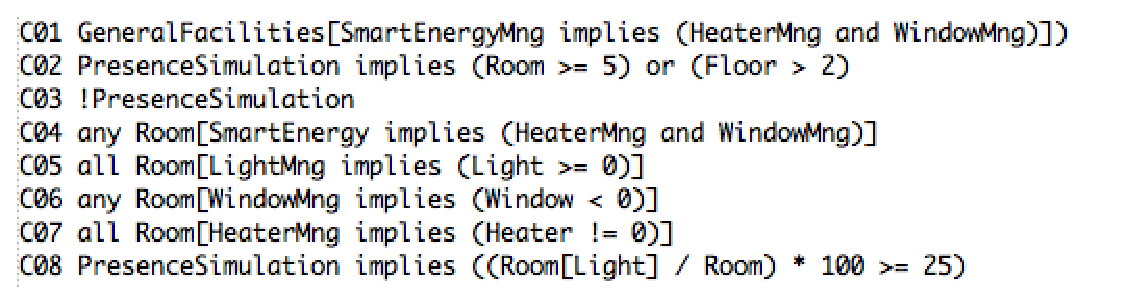
\includegraphics[scale=0.6]{metamodelo/instpruebas.eps}
    \caption{Conjunto de instrucciones que puso a prueba el funcionamiento del metamodelo}
    \label{figmetains}
\end{figure}

Las instrucciones que fueron puestas a prueba fueron las que se ven en la Figura~\ref{figmetains}. Este conjunto de instrucciones servir�n como pruebas tambi�n en momentos m�s avanzados del desarrollo. Dicho conjunto de pruebas fue dise�ado para recoger de la forma m�s exhaustiva posible todas las combinaciones de metaclases posibles.
